\section{Polynome und weitere elementare Funktionen}\label{sec:polynome}

\begin{definition}{Polynom}
    Eine Polynomfunktion ist eine Funktion der Form: \[y = f(x) = a_n \cdot x^n + a_{n-1} \cdot x^{n-1} + \cdots + a_1 \cdot x + a_0\] mit $a_n \neq 0$, wobei $n$ der \emph{Grad} und $a_0, a_1, \dots, a_n \in \R$ die \emph{Koeffizienten} der Polynomfunktion darstellen.
\end{definition}

\subsection{Das Horner-Schema und der Zerlegungssatz}\label{subsec:horner-schema}

\textbf{Gegeben:} Eine Polynomfunktion $f(x) = a_{n}x^n + a_{n-1}x^{n-1} + \dots + a_{1}x + a_0$.

\textbf{Ziel:} Zu einem gegebenen $x_0$ (z.B. $x_0 = -2$) möglichst effizient den Wert $f(x_0)$ ausrechnen.

\textbf{Variante 1:} Für jedes $k$ den Ausdruck $a_{k}x^{k}$ bestimmen (braucht $k$ Multiplikationen).

$\Rightarrow$ \textbf{Aufwand:} $\quad n + n - 1 + \dots + 2 + 1 + 0 = \frac{n \cdot (n+1)}{2} \quad$
Für $n=10$ werden 55 Multiplikationen benötigt!

\textbf{Variante 2:} Das Horner-Schema verwenden.
Hierbei werden die Terme umgeformt, damit Multiplikation schrittweise erfolgen kann.
Für ein Polynom vom Grad 4:

$\Rightarrow$ \textbf{Aufwand:} $\quad ((((a_4) \cdot x + a_3) \cdot x + a_2) \cdot x + a_1) \cdot x + a_0 \quad$ Anzahl Multiplikationen: 4.

\textbf{Allgemein:} Für ein Polynom vom Grad $n$ werden $n$ Multiplikationen benötigt.
Für $n = 10$ werden also 10 Multiplikation benötigt (statt 55).

\subsubsection{Horner-Schema für Polynom-Auswertung}

Das Schema von Horner biete eine übersichtliche Art, ein Polynom auf diese effiziente Weise auszurechnen.
Veranschaulichung anhand des Beispiels: \[f(x) = 3x^4 - 2x^3 + 5x^2 - 7x - 12\]

\vspace{-\topsep}

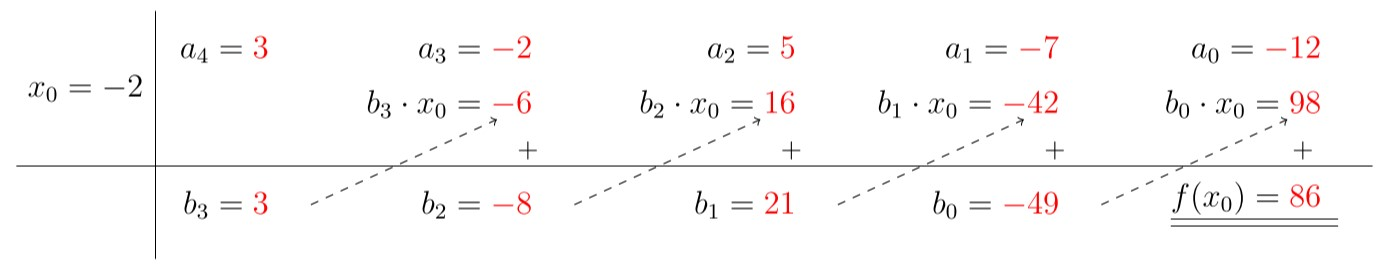
\includegraphics[scale=0.5]{horner-schema}

\subsubsection{Zerlegungssatz}

\begin{definition}{Zerlegungssatz (ohne Beweis)}
    Ist $x_0$ eine Nullstelle der Polynomfunktion $f(x)$, dann gibt es eine bestimmte Polynomfunktion $g(x)$ so dass \[f(x) = (x - x_0) \cdot g(x)\] für jedes x.
\end{definition}

\textbf{Bemerkung:} Der Faktor $(x - x_0)$ heisst Linearfaktor. $g(x)$ ist das sogenannte \emph{1. reduzierte Polynom}: Der Grad von $g(x)$ ist um 1 kleiner als der Grad von $f(x)$.

\subsubsection{Nullstellen von Polynomfunktionen}

\begin{definition}{Satz}
    Eine Polynomfunktion vom Grad $n$ hat höchstens $n$ Nullstellen.
    $x_0$ heisst \emph{m-fache Nullstelle} der Polynomfunktion $f(x)$, falls es eine bestimmte Polynomfunktion $g(x)$ gibt, so dass \[f(x) = (x - x_0)^m \cdot g(x)\] für jedes $x$.
\end{definition}

\subsection{Division von Polynomen}\label{subsec:division-von-polynomen}

Mithilfe des Horner-Schemas können Polynome nur durch \emph{lineare} Faktoren (d.h. Polynome vom Grad 1) dividiert werden.
Zum Beispiel:

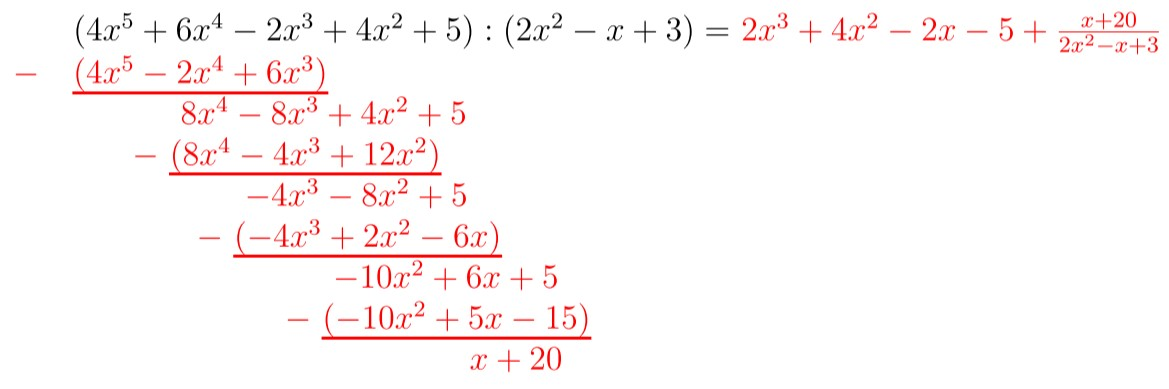
\includegraphics[scale=0.5]{polynom-division}